\chapter{Implementierung / Design}

In diesem Kapitel wird die Implementierung des Plan Generators näher erläutert. Begonnen wird mit 5 Design-Prinzipien, die für die Entwicklung zum Einsatz gekommen sind. Sie erlauben es den Plan Generator schnell zu erweitern, Adaptoren für externe Systeme herzustellen und so die Erweiterbarkeit zu garantieren.


\section{SOLID Prinzipien}

Das Projekt wurde nach den SOLID-Design-Prinzipien \cite{unclebob1995} aufgebaut. SOLID steht für Single responsibility, Open-closed, Liskov substitution, Interface segregation and Dependency inversion. Es sind  eine Menge von Prinzipien, die bei der objektorientierten Programmierung zum Einsatz kommen und durch deren Anwendung die Wartbarkeit und Erweiterbarkeit des Codes erhöht werden soll. Alle fünf Prinzipien finden Anwendung in der Implementierung.

\begin{itemize}
\item Das Prinzip der Single Responsibility  ist auch unter dem Namen Kohäsion bekannt. Es sagt aus, dass eine Klasse immer nur eine Verantwortlichkeit besitzt.  Potenzielle Anforderungsveränderungen lassen sich schnell umsetzen, da potenziell nur eine Klasse von einer solchen Änderung betroffen ist.

\item Das Open/closed Prinzip sagt aus, dass Klassen für Erweiterung offen, jedoch verschlossen für Modifikation sein sollen. Dieses Prinzip erlaubt es Änderungen an einer übergeordneten Klasse durchzuführen, die automatisch von allen untergeordneten Klassen übernommen werden können. Gemeinsame Codebasen verringern den Entwicklungsaufwand und erleichtern die Erweiterung.

\item Das Liskov substitution Prinzip sagt aus, dass eine Klasse, die von einer anderen Klasse erbt, sich genau so verhalten soll wie es von der übergeordneten Klasse erwartet wird. Die Instanz eines Subtypen sollte sich von außen betrachtet also genau so verhalten, wie eine Instanz des Haupttypen.

\item Das Interface-Segregation-Prinzip dient zur Aufteilung von Interfaces. Es ist dabei besser für jeden Anwender einer Klasse ein eigenes Interface zu erstellen, das genau die Funktionen abbildet, die von einem Anwender verwendet werden, als eine großes Interface zu erstellen, das von allen Anwendern genutzt werden kann. So kann der Überblick über verschiedene Anwender besser behalten werden.

\item Das Dependency-Inversion-Prinzip sorgt für die Reduktion von Abhängigkeiten über verschiedene Komponenten eines Systems. Konkret schlägt das Prinzip vor, dass High-Level Module nicht abhängig von low-level Modulen sein sollten.

\end{itemize}

Jedes der vorgestellten Prinzipien gibt eine Leitlinie vor, mit deren Hilfe ein hohes Maß an Zuverlässigkeit, Wartbarkeit und Verständlichkeit erzielt werden kann. Nur wenn alle Prinzipien gleichermaßen zur Anwendung kommen, können diese Qualitäten gesteigert werden. Die im Weiteren beschriebene Implementierung fußt auf diesen fünf Prinzipien. In jedem Modul, jeder Klasse und jeder Methode wurde auf die Anwendung der Prinzipien geachtet.

\section{Notation und Style Guide}
Um ein einheitliches Bild der Implementierung zu wahren wurde bei der Implementierung streng auf die Einhaltung der Formatierungsrichtlinien anch \"Allman\".

Immer wieder im folgdenden Code tauchen Typen auf, die mit dem Postfix \texttt{\_t} 

\section{Der Optimierungsvorgang}

\begin{figure}[h]
  \centering
  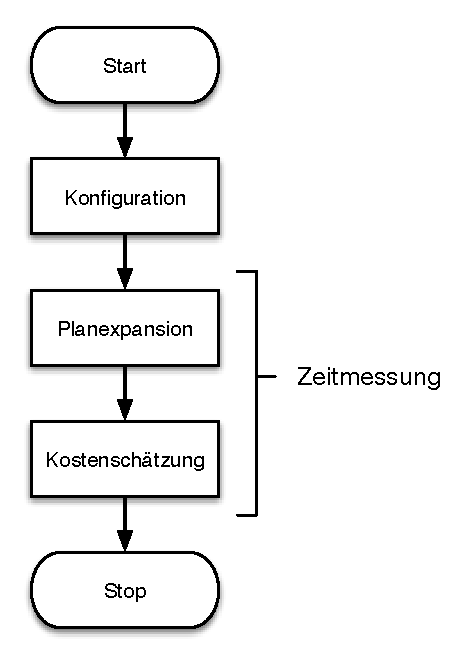
\includegraphics{04_Implementierung/00_media/Ablauf.pdf}
  \caption{Ablauf der eigenen Implementierung}
  \label{Ablauf}
\end{figure}

Die Ausführung des Programms geschieht in drei Schritten (vgl. Abb. \ref{Ablauf}): (1) Konfiguration, (2) Generierung von semantisch gleichen Plänen, (3) Finden des optimalen Plans.




Im ersten Schritt, wird auf Grund von externen Parametern das System konfiguriert. Die Konfiguration erfolgt durch ein JSON File. In ihm werden die Parameter (Relationen und deren Kardinalität, Join-Kanten und deren Selektivität, initialer Plan und Regelmengen) für die Optimierung festgelegt. Mit Hilfe der Relationen und deren Kardinalität können später im Zusammenspiel mit Join-Kanten und Selektivität die Kosten für einen Plan berechnet werden. Der initiale Plan dient als Startpunkt der Transformation. Auf ihn werden die Regelmengen angewendet und so logische  Äquivalente erzeugt.

Zu Beginn des zweiten Schritts, der Erzeugung von äquivalenten Plänen, wird die Zeitmessung gestartet.  Mit Hilfe von Enumeratoren werden die unterschiedlichen Regelmengen auf den initialen Plan angewendet.

In einem finalen Schritt findet die Kostenberechnung statt um aus den möglichen Plänen den günstigsten auszuwählen. Diese Preisberechnung wird im Modul der Kostenschätzung vollzogen.



\begin{figure}[ht]
  \centering
  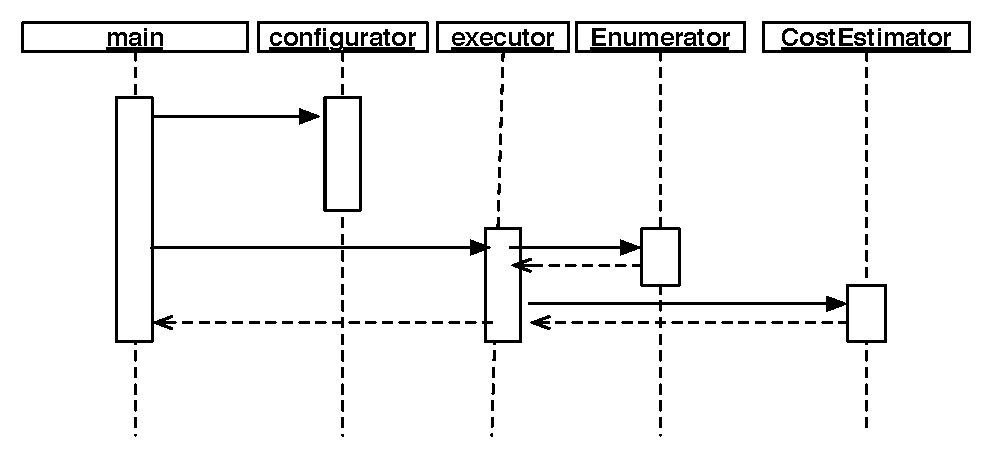
\includegraphics[width=\textwidth]{04_Implementierung/00_media/SequenceDiagramConfiguration.pdf}
  \caption{Sequenzdiagramm: Aufruf der einzelnen Komponenten}
  \label{SequenceDiagramConfiguration}
\end{figure}


Die genaue Reihenfolge der Aufrufe beginnend mit der Hauptmethode lässt sich in Abbildung \ref{SequenceDiagramConfiguration}, einem Sequenzdiagramm, am besten ablesen. Zuerst muss die Konfiguration abgefragt werden. Diese Konfiguration wird dann an einen Exektor weitergegeben, der für Zusammenstellung von Regelmengen und Enumerator verantwortlich ist, ebenfalls ruft er die Kostenschätzung auf und ruft die Zeitmessung auf. Die einzelnen Komponenten werden im Folgenden genau besprochen.

\section{Services}
\subsection{Zeitmessung}

\begin{figure}[ht]
  \centering
  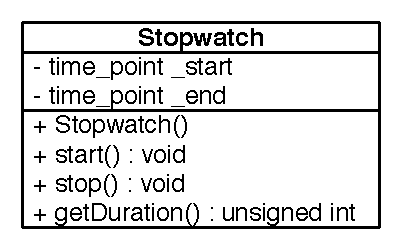
\includegraphics[scale=0.75]{04_Implementierung/00_media/Stopwatch.pdf}
  \caption{Klassendiagramm: Stopwatch}
  \label{ClassStopwatch}
\end{figure}

Wie bereits in Abb. \ref{Ablauf} dargestellt, wird die Zeitmessung, die durch die Klasse Stopwatch (vgl. Abb. \ref{ClassStopwatch}) durchgeführt wird, nach der Konfiguration zuerst instantiiert und dann mit der Methode \texttt{start()} gestartet. Sobald alle Pläne expandiert und die Kosten berechnet sind, wird die Messung durch die Methode \texttt{stop()} beendet. Um eine möglichst genaue Messung durchführen zu können, wurde die Uhr \texttt{std::chrono::steady\_clock} verwendet. Diese Uhr ist Teil von C++11. Wie in der Dokumentation \cite{cppreference_2015_clock} beschrieben, handelt es sich dabei um eine monotone Uhr. Sie kann nicht rückwärts laufen, solange die physische Zeit fortfährt. Die Uhr selbst mit der Wall\-Clock\-Time verbunden, ist das passende Werkzeug zur Messung von Intervallen. 

Die Dauer zwischen dem Start der Expansion und dem Ende der Kostenberechnung wird in Nanosekunden gemessen und mit der Methode \texttt{getDuration()} ausgegeben, um ein möglichst akkurates Ergebnis zu erhalten. Die gemessenen Ergebnisse werden sowohl als Debug-Log in der Konsole ausgegeben, als auch  in einem Log File gespeichert.




\subsection{Logging und Debugging}
Zum Debugging wurde auch eine externe Bibliothek eingesetzt: EasyLogging++ \cite{easylogging}, ein einfach zu bedienendes, jedoch hochgradig konfigurierbares Logging Instrument. Gerade die Leichtgewichtigkeit - das Tool besteht nur aus einer Headerklasse -, die einfache Bedienung und die Geschwindigkeit gaben  den Ausschlag zur Nutzung der Library. Mit Hilfe dieser Library werden debugging Informationen geschrieben, aber auch Zeitmessungen gespeichert, Pläne ausgegeben und sonstige Debugging Nachrichten ausgegeben. Insbesondere ist die Unterscheidung zwischen unterschiedlichen Debug\-Leveln wichtig. Auf mehreren Ebenen (INFO, WARNING, DEBUG, etc.) können Informationen ausgegeben werden. Je nachdem welches Level angesprochen ist, werden nur Informationen darüber ausgegeben. 

\subsection{Operatoren und Operations}
Wie in Abb. \ref{PlanNodeClass} zu sehen, sind zwei Operatoren vorgesehen JOIN und SCAN. Um aus ihnen im Zusammenhang mit Planknoten und Äquivalenzklassen Pläne herzustellen, wurde die Klasse \texttt{Operations} (vgl. \ref{ClassOperations} erstellt. Diese Klasse bietet einfachen Zugriff auf die meist verwendeten Arten von Äquivalenzklassen und Planknoten. Beispielsweise kann mit der Methode \texttt{scan} direkt eine Äquivalenzklasse mit einer bestimmten Relation, ein übergeordneter Planknoten und eine wiederum übergeordnete Äquivalenzklasse erstellt werden.

Neben diesem Operator steht auch ein Oprator zur Erzeugung von Joins mit und ohne übergeordneter Äquivalenzklasse zur Verfügung \texttt{join} resp. \texttt{joinPN}.

Um Kosten bei der Erzeugung neuer Objekte zu sparen, werden alle Planknoten und Äquivalenzklassen in Resourvars angelegt. Es werden also bereits vor dem Start des eigentlichen Tests alle Instanzen gebildet und während der Laufzeit mit konkreten Daten gefüllt.



%\input{04_Implementierung/Organisation.tex}
\section{Konfiguration}


\begin{figure}[ht]
  \centering
  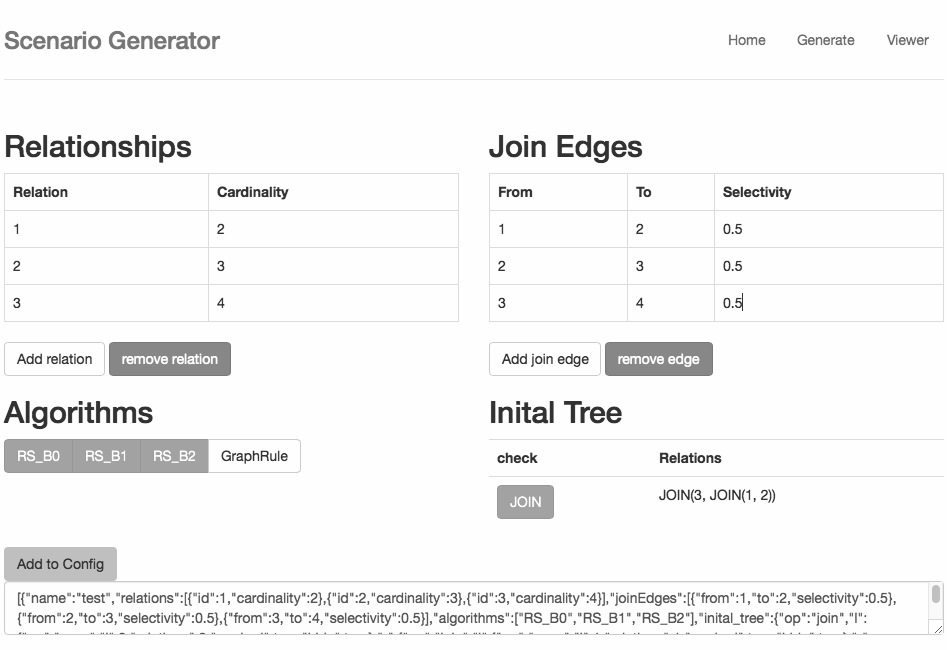
\includegraphics[width=1\textwidth]{04_Implementierung/00_media/Tool.png}
  \caption{Konfigurationstool: Scenario-Generator}
  \label{ScenarioGenerator}
\end{figure}

Das Konfigurationsmodul besteht aus zwei Komponenten. Auf der einen Seite eine Javascript-HTML Anwendung zur Generierung von Test-Szenarien (vgl. Abb. \ref{ScenarioGenerator}). Mit Hilfe dieser Anwendung können Konfigurationsfiles für den späteren Test erstellt werden. Dieses Konfigurationssystem, das in  zu sehen ist, bietet dem Nutzer die Möglichkeit Relationen mit Kardinalitäten zu erzeugen, Selektivitäten festzulegen und schlussendlich einen initialen Plan zu erzeugen. Ebenfalls ist es möglich die verschiedenen Regelmengen, die geprüft werden sollen, festzulegen.

Das Ergebnis dieses Moduls ist eine Konfigurationsdatei im JSON-Format. Das Tool unterstützt die Erzeugung mehrerer Szenarien in einem Konfigurationsfile. So können mehrere Szenarien in einem Test-Run durchgespielt werden. Die Verwendung des JSON-Formats bietet viele Vorteile. U.a. waren die folgenden Vorteile ausschlaggebend für die Verwendung von JSON:

\begin{itemize}
\item Im Gegensatz zu XML ist JSON einfacher. Weniger Grammatik ist vorhanden.
\item Das Format ist hoch Interoperable und kann nativ von Javasciript ausgegeben werden. Ebenfalls ist es möglich mit Hilfe von einfachen Parsern JSON in C++ zu verarbeiten.
\item JSON ist durch die einfache, jedoch standardisierte Form leicht für Menschen zu lesen und Fehler sind leichter aufzuspüren.
\item Das gewählte Format zur Repräsentation der unterschiedlichen Parameter ist einfach erweiterbar. Attribute und neue Objekte können jederzeit hinzugefügt werden.
\end{itemize}

\subsection{Aufbau und Funktion der Konfigurationsdatei}

Ein konkretes Test File ist in \ref{JsonConfigFile} zu sehen. Jedes Test File ist ein Array von Test-Objekten. Für jeden Test wird mit dem Attribut \texttt{name} ein Name gespeichert. Für jede Relation, die in einem Test vorkommt, wird ein Relations-Objekt erzeugt. Es besteht aus einer \texttt{id}, der Relations-Id, und der dazugehörigen Kardinalität. Mehrere dieser Relations-Objekte werden in einem Array gespeichert und sind dem \texttt{relation}-Attribut des Test-Objekts zugewiesen. Im konkreten Fall sind zwei Relationen vorhanden. Eine mit der \texttt{id:1} und eine mit der \texttt{id:2} 2. Für Beide wurde eine Kardinalität zugewiesen. 

Auch für Join-Kanten werden Objekte erzeugt. Ein Join-Kanten Objekt bezeichnet eine Kante zwischen zwei Relationen. Eine Kante könnte, wie im Beispiel zu sehen von der Relation 1 zu der Relation 2 verlaufen, wobei die Richtung nicht entscheidend ist. Einer Join-Kante wird auch eine Selektivität zugeordnet. Mehrere dieser Join-Edge-Objekte werden als Array im Attribut \texttt{joinEdges} hinterlegt.

Neben Join-Kanten und Relationen sind auch die zu testendeden Algorithmen gespeichert. Sie werden in einem Array abgelegt und sind dem Attribut \texttt{algorithms} zugewiesen. Im vorliegenden Beispiel werden die Regelsets \texttt{RS-B0}, \texttt{RS-B1} und \texttt{RS-B2} getestet.

Auch ein initialer Plan wird im Test-Objekt gespeichert. Ein Baum besteht immer aus Knoten. Für jeden Knoten wird ein Operator im Attribut \texttt{op} gespeichert. Es wird der Operator \texttt{SCAN} und der Operator \texttt{JOIN} unterstützt. Ein Knoten kann eine linke und eine rechte Seite haben. In Zeile 14 ist eine Scan Operation zu sehen. Es wird nur die linke Seite verwendet. Im Attribut \texttt{l} ist die ID der Relation abgelegt, die zu scannen ist. Bei \texttt{JOINs} wird auch die rechte Seite verwendet (vgl. Zeile 16). In den Attributen \texttt{l} und \texttt{r} können entweder weitere Knoten oder Relations-Ids gespeichert werden. Neben Operator, links und rechts ist das Attribut \texttt{relations} Teil des Knotens. Hier ist eine einfache Repräsentation des Knotens gespeichert. Im Falle von Zeite 14 \texttt{1}. sind komplexere Knoten und Subknoten vorhanden, können komplexere Daten im Feld \texttt{Relations} abgelegt sein. Beispielsweise ist eine solche komplexere Form in Zeile 19 ( \texttt{JOIN(1,2)}) zu erkennen. Hier ist ein Join zwischen 1 und 2 zu sehen.

\begin{minipage}{\linewidth}
\lstinputlisting[caption=JSON: Konfigurations-File, label=JsonConfigFile]{04_Implementierung/00_media/config.json}
\end{minipage}

\subsection{Konfiguration eines Test innerhalb des Prototypen}

Die eigentliche Konfiguration findet in C++ statt. Mit der Bibliothek json11 \cite{json11} wird das Konfigurationsfile gelesen. Dieser Vorgang wird von der Klasse \texttt{Config\-urator} übernommen. Auf Basis eines Dateipfades zu einer Konfigurationsdatei erzeugt die Klasse einen Vektor von \texttt{Configuration} Instanzen. Für jedes JSON Test-Objekt wird eine solche Konfigurationsinstanz erzeugt und die für die Konfiguration notwendigen Informationen hinterlegt.

Jedes Konfigurationsobjekt (vgl. Abb. \ref{Konfiguration}) bietet eine Menge unterschiedlicher Methoden an, um Informationen über den aktuellen Test zu erlangen.

Mit Hilfe der Methode \texttt{getInitaleTree()} wird ein Baum aus Äquivalenzklassen und Planknoten erzeugt, die den initalen Plan erzeugen. Die Methode erzeugt immer eine neue Instanz des gesamten Baums.

Die Kardinalität und Selektivität, die als ausschlaggebende Kennzahlen zur Berechnung des optimalen Plans herangezogen werden, sind mit den Methoden \texttt{get\-Cardinaility()} und \texttt{get\-Selectivity()} zu erfragen. Auch die getesteten Algorithmen können mit der Methode \texttt{getAlgorithms()} ausgelesen werden.


\begin{figure}[ht]
  \centering
  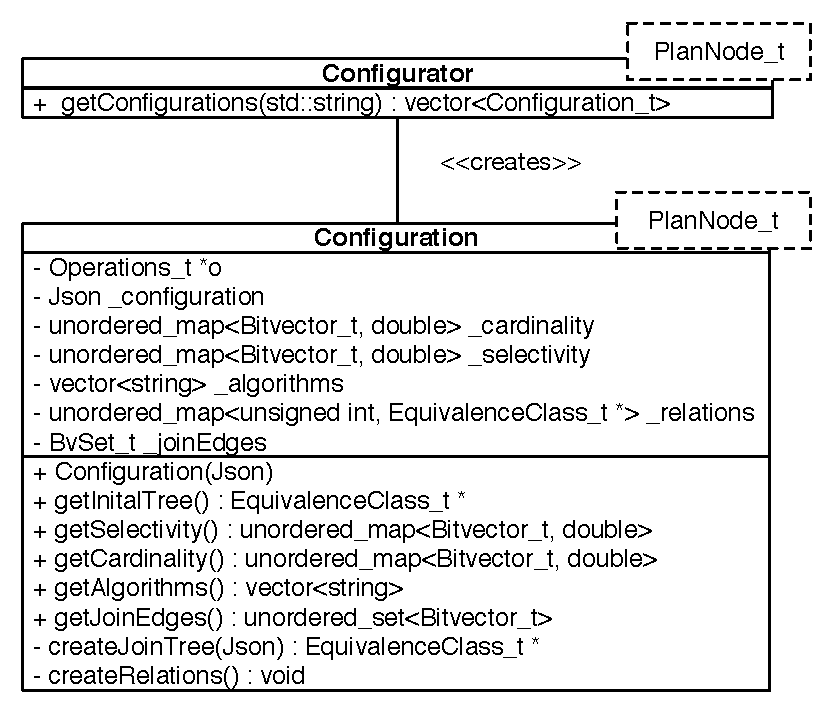
\includegraphics[width=0.75\textwidth]{04_Implementierung/00_media/ConfigurationClass.pdf}
  \caption{Klassendiagramm: Konfiguration}
  \label{Konfiguration}
\end{figure}

\section{Knoten und Äquivalenzklassen}

\subsection{Repräsentation von Relationen}
\label{sec:Bitvector}

Die einzelnen Relationen werden mit Hilfe eines Bitvektors dargestellt. Jeder Basis-Relation - sie repräsentiert eine physische Relation - ist eine ID zugeordnet. Eine Basis-Relation wird in diesem Prototypen mit Hilfe eines auf \texttt{TRUE} gesetzten Bits in einem Bitvektor repräsentiert. Auch mehrere Relationen können durch einen Bitvektor abgebildet werden dazu werden mehrere Bits auf \texttt{TRUE} gesetzt.

\subsubsection{Implementierung}

Als Basis für die Implementierung dient ein Bitvektor. Ein Bitvektor sind mehrere Bits, die entweder \texttt{TRUE} also \texttt{1} oder \texttt{FALSE} also \texttt{0} sein können. Ist das n-te Bit eines Bitvektors gesetzt, so repräsentiert dieses Bit die n-te Relation. Beispielsweise bezeichnet der Bitvektor \texttt{010000000} die Relation mit der ID \texttt{1}. Mit Hilfe des Bitvektors können auch mehrere Relationen gespeichert werden \texttt{01010000000} bezeichnet folglich die Relation mit dem Name \texttt{1} und die Relation mit der ID \texttt{3}. Für die durchgeführten Berechnungen ist es nicht notwendig, dass eine Relation mit ihrem tatsächlichen Namen bekannt ist. Es reicht eine Bezeichnung mit Hilfe von Nummern aus.

Vorteil für die Verwendung von Bitvektoren ist, dass einfach Mengenoperationen durchgeführt werden können. So kann einfach geprüft werden, ob Äquivalenzklassen gemeinsame JOIN Kanten besitzen oder neue Relationen einer Äquivalenzklasse hinzugefügt werden. (vgl. Abb. \ref{Bitvector}) Dies ist besonders effizient, da nur Bits und keine komplexen Objekte wie Strings verarbeitet werden müssen.



\begin{figure}[ht]
  \centering
  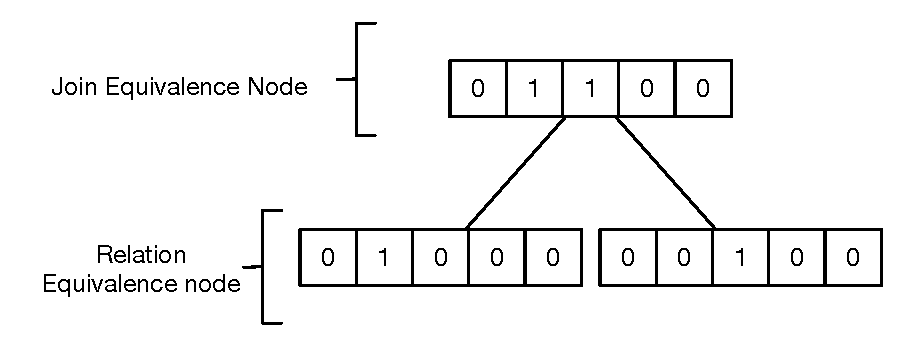
\includegraphics{04_Implementierung/Bitvector.pdf}
  \caption{Bitvekotren als Repräsentation von Relationen oder Joins}
  \label{Bitvektor}
\end{figure}


Die konkrete Erzeugung von Bitvektoren zu repräsentation von Relationen entsteht bei der Erstellung neuer Pläne bzgl. Äquivalenzklassen. Bezeichnet eine Äquivalenzklasse nur eine Basis-Relation so ist ihr Bitevektor \texttt{\_relations} auf nur einen Wert gesetzt. Wird einer Äuqivalenzklasse ein Planknoten hinzugefügt, wird die Variable \texttt{\_relations} mit den Relationen, die links bzw. rechts an einem Plan-Knoten hängen angereichert.



\subsubsection{Erweiterbarkeit}
Die Implementierung des Bitvektors erlaubt es mit Hilfe eines Templateparameters die Länge des Bitevektors anzupassen.



\subsection{Planknoten und Äquivalenzklassen}




\begin{figure}[ht]
  \centering
  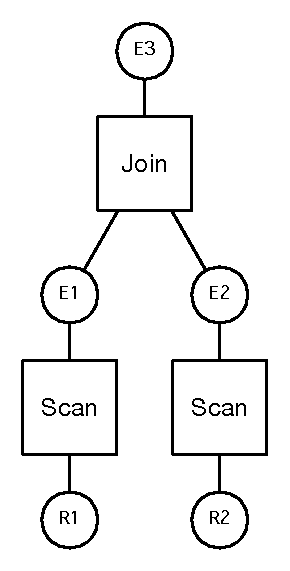
\includegraphics{04_Implementierung/JoinScan.pdf}
  \caption{Planknoten und Äquivalenzklassen}
  \label{PlanAequi}
\end{figure}

Die Datenstruktur in der Pläne gespeichert sind sind sowohl \texttt{Plannode} und \texttt{EquivalenceClasses}. Einem Planknoten ist ein Operator zugewiesen. Beispielsweise \texttt{JOIN} oder \texttt{SCAN}. In \texttt{EquivalenceClass} werden mehrere Pläne gespeichert, die alle semantisch gleich sind. Ein einfaches Beispiel ist in Abbildung \ref{PlanAequi} zu finden. Ein einfacher Plan bestehend aus einem Join und zwei Scans ist zu sehen. Der oberste Knoten \texttt{E3} ist eine Äquivalenzklasse in Ihr findet sich der erste Planknoten ein Join. Der Join hat zwei Seiten eine linke und eine rechte. Beide Seiten sind mit einer Äquivalenzklasse verbunden \texttt{E1} resp. \texttt{E2}. Die jeweils einen Scan beinhalten, der die Basis-Relationen \texttt{R1} bzw. \texttt{R2} einliesst. Die Beiden Basis-Relationen sind ebenso wie die Äquivalenzklassen als \texttt{EquivalenceClass} im System abgelegt.




\subsubsection{Implementierung}

\begin{figure}[ht]
  \centering
  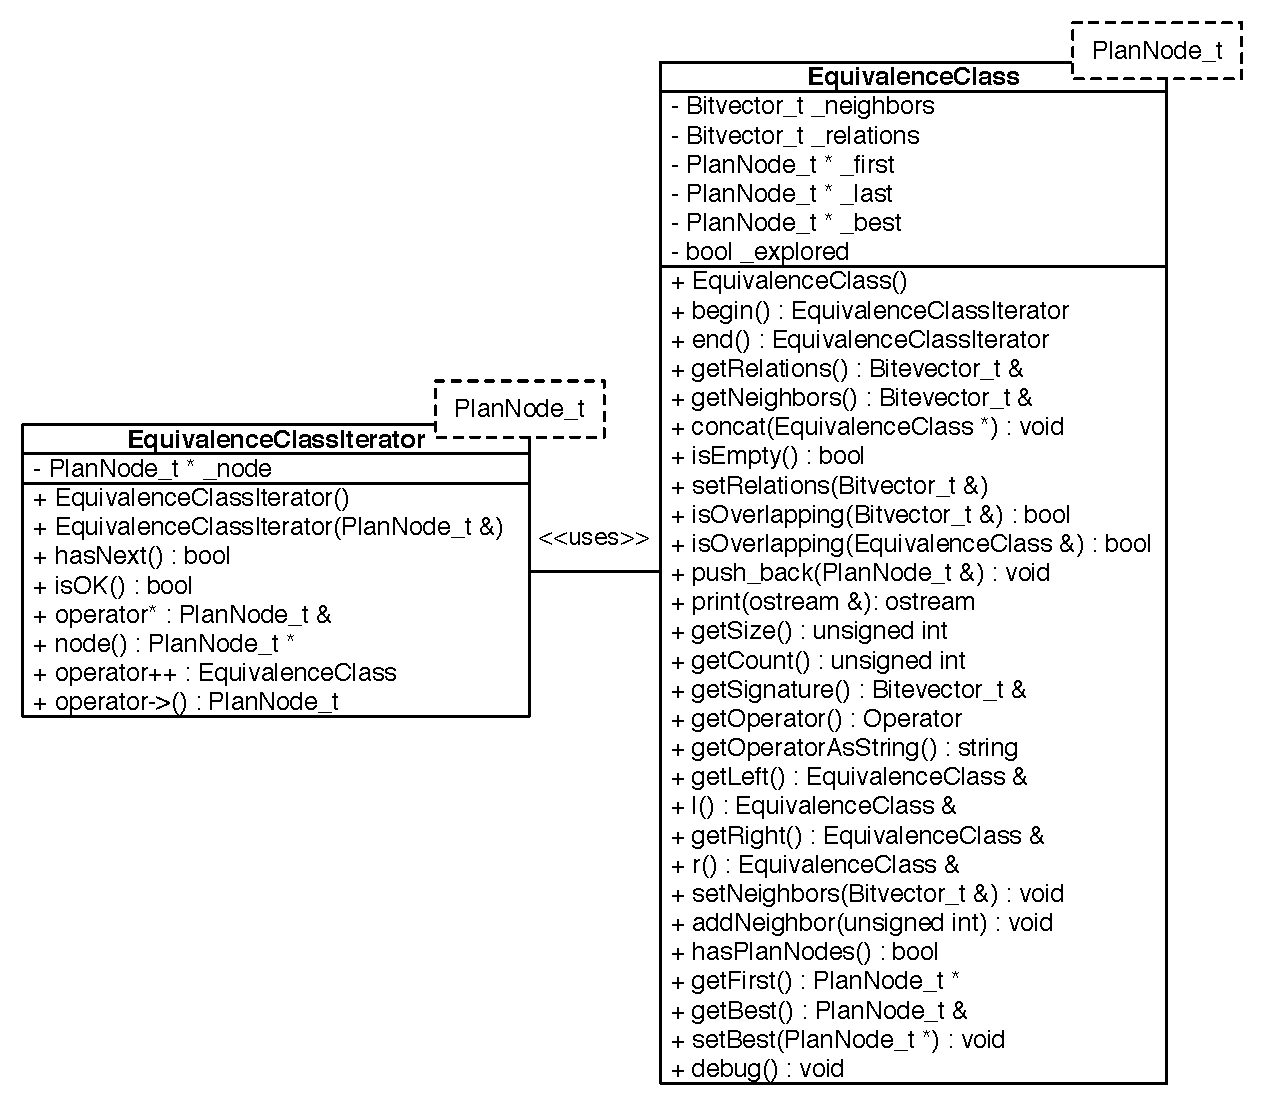
\includegraphics[width=1\textwidth]{04_Implementierung/ClassEquivalenceClass.pdf}
  \caption{Klassendiagramm: Äquivalenzklasse}
  \label{ClassEquivalenceClass}
\end{figure}

\subsubsection{Erweiterbarkeit}


\section{Regeln und Regelmengen}
Auf die Planknoten müssen während der Enumeration Regeln angewendet werden. Diese Regeln sind im vorliegenden Prototypen als \texttt{Rules} und \texttt{Regelmengen} abgelegt.

\subsection{Regelmengen}
Mehrere Regeln werden in einer Regelmenge zusammengefasst.
Insgesamt wurden vier unterschiedliche Regelmenegen implementiert: \textit{RS-B0}, \textit{RS-B1}, \textit{RS-B2} und \textit{GraphRule}.
Alle Mengen basieren auf den von Pellenkoft et al. vorgestellten Regelmengen und dem von \cite{shanbhag2014optimizing} implementierten GraphRule.

\begin{figure}[ht]
  \centering
  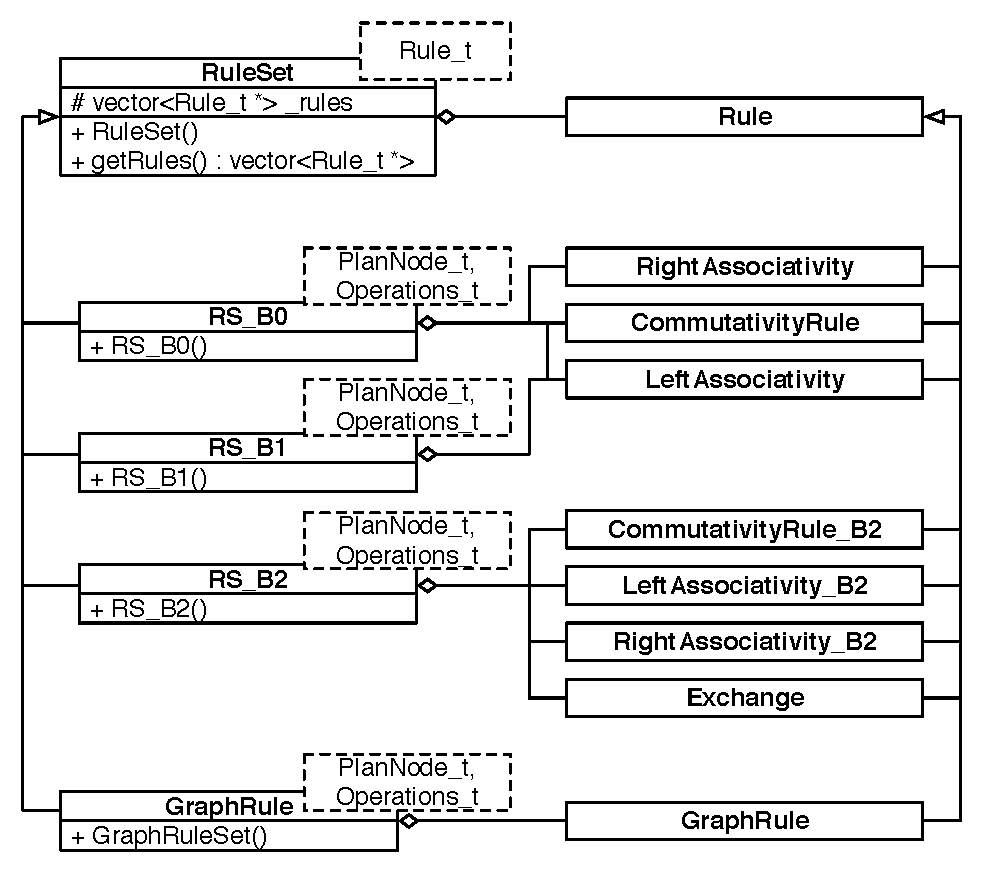
\includegraphics[scale=0.75]{04_Implementierung/00_media/RuleSets.pdf}
  \caption{Klassendiagramm: Regelmengen und Regeln}
  \label{RuleSetClass}
\end{figure}

\subsubsection{Implementierung}
\label{sec:RuleImplementation}

Alle Regelmengen erben von der Klasse \texttt{RuleSet}, die die Methode \texttt{getRules()} implementiert, mit deren Hilfe ein Vektor von Regeln ausgegeben wird. Je nach Regelmenge können andere Regeln vorhanden sein. Eine Übersicht über Regeln und deren Zuordnung zu Regelsets findet sich in Abb. \ref{RuleSetClass}.

Die einzelnen Regeln bei der Erstellung einer Regelmenge instantiiert, sind dem Vector \texttt{\_rules} zugeordnet. Die Sammlung der Regeln in einem Vector ist möglich, da alle Regeln von der abstrakten Klasse \texttt{Rule} erben. 

Konkret ist dem Regelset \textit{RS-B0} die Regel \texttt{RightAssociativity}, \texttt{Commutativity} und \texttt{LeftAssociativity} zugeordnet, dem Regelset \textit{RS-B1} \textit{Left Associativity} und \textit{Commutativity}. Dem Regelset \textit{RS-B2} sind die Varianten von Kommutativität, linker und rechter Assozativität, die speziell für diese Regelmenge erstellt wurden, zugeordnet, ebenso wie die \texttt{Exchange} Regel. Der \textit{Graph Rule} wird nur für \textit{RS-Graph} benötigt.

\subsubsection{Erweiterbarkeit}
Die Erweiterung der Regelmengen ist in verschiedenen Dimensionen möglich. Neue Funktionen können für die Regelmengen implementiert werden, ebenso ist die Erstellung neuer Regelmengen möglich.

Auf funktionaler Ebene ist es vorstellbar, dass die Reihenfolge der Regeln dynamisiert werden. Aktuell ist es nur möglich, die Regeln in Form eines Vektors auszugeben, dessen Reihenfolge immer gleich ist. Da alle konkreten Regelmengen von der selben Klasse \texttt{RuleSet} erben, ist die Implementierung einer anpassbaren Reihenfolge leicht möglich und muss für alle Klassen nur einmal vorgenommen werden.


Auch das Hinzufügen von neuen Regeln zu bestehenden Regelmengen oder die Erweiterung von bestehenden Regelmengen ist möglich. Beispielsweise kann von bestehenden Regelmengen geerbt wird bzw. neue Regeln und deren Regelmengen durch die Implementierung der standardisierten Interfaces \textit{RuleSet} entstehen.

Die Erweiterbarkeit konnte mit der Implementierung der Regelmenge  \textit{Graph Rule} unter Beweis gestellt werden, da diese Regelmenge erst später entwickelt wurde und auf die bestehende Infrastruktur aufsetzte.




\subsection{Regeln}

\begin{figure}[ht]
  \centering
  \includegraphics[scale=0.75]{04_Implementierung/00_media/Rules.pdf}
  \caption{Klassendiagramm: Regeln}
  \label{RuleClassDiagram}
\end{figure}

Die einzelnen Regeln, die Teil der Regelmengen sind, werden jeweils in einer eignen Klasse abgelegt. Aktuell sind acht Regeln vorhanden: (1) \texttt{Commutativity}, (2) \texttt{Left Associativity}, (3) \texttt{Right\-Associativity}, (4) \texttt{Commu\-tativity B2}, (5) \texttt{Left\-Associtativity-B2}, (6) \texttt{Right\-Associativity-B2}, (7) \texttt{Exchange}, (8) \texttt{Graph Rule}. Die Zuordnung der Regeln zu den unterschiedlichen Regelmenegen wurde in \ref{sec:RuleImplementation} erklärt und in Abb. \ref{RuleSetClass} veranschaulicht.

Einer der konzeptionellen Unterschiede zwischen den in Kapietl 3 beschriebenen Regeln und den hier implementierten Regeln ist, dass die hier implementierten Regeln per se kreuzproduktfrei sind. Es wird bereits vor der Anwendung einer Regel geprüft, ob eine Regel ein Kreuzprodukt generieren wird, nur wenn das Ergebnis kreuzproduktfrei sein wird, kommt die Regel zur Anwendung. Dieses Vorgehen ermöglicht,  bereits frühzeitig die Generierung von Plänen abzubrechen, wenn die erzeugten Pläne nicht zielführend sind. Da die Regeln nicht prüfen, ob nach ihrer Anwendung ein Kreuzprodukt entstanden ist, sondern diese Prüfung bereits zuvor geschieht, werden die Regelmengen im Folgenden auch nicht mit dem Post-Fix -CPS bezeichnet.

\subsubsection{Implementierung}


\begin{figure}[ht]
  \centering
  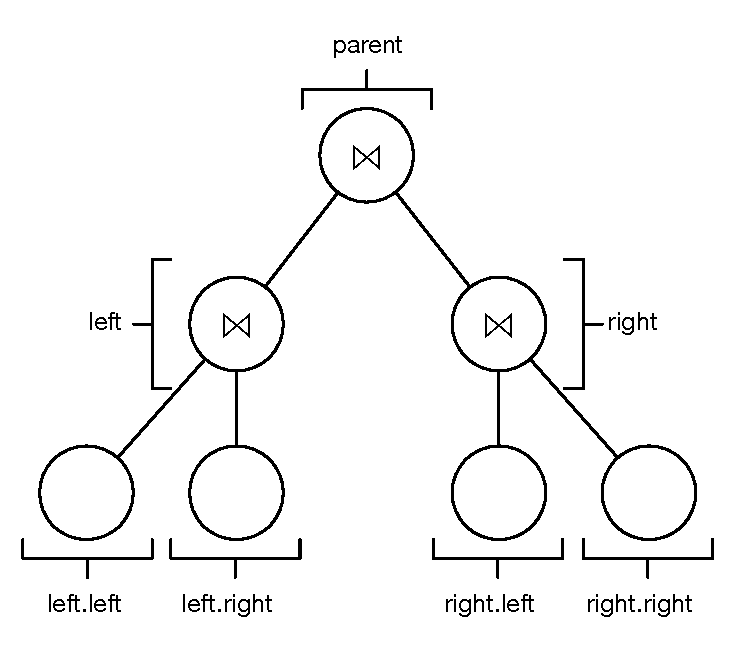
\includegraphics[scale=0.75]{04_Implementierung/00_media/Plan.pdf}
  \caption{Plandiagramm: Einfacher Beispiel-Plan}
  \label{SimplePlan}
\end{figure}


Auch bei den Regeln erben alle Regeln direkt oder - und das ist neu - indirekt von der Klasse \texttt{Rule}. Die Organisation der Klassen ist in Abb. \ref{RuleClassDiagram} dargestellt. Alle Regeln implementieren das Interface, das durch die abstrakte Klasse \texttt{Rule} vorgegeben ist. Durch die Methode \texttt{getName()} wird der Name der jeweiligen Regel zurückgeliefert. Wie bei anderen Implementierungen sind die Regeln in zwei Teilen organisiert. Mit Hilfe der Methode \texttt{isApplicable} kann festgestellt werden, ob eine Regel anwendbar ist, Die Methode \texttt{apply} wendet die Regel an und liefert einen Planknoten zurück. Kreuzprodukte werden nicht wie bei \cite{shanbhag2014optimizing} erst nach der Bildung neuer Pläne geprüft, sondern schon im \texttt{isApplicable}-Teil. So werden ausschließlich kreuzproduktfreie Bäume gebildet. Der Planknoten selbst, sowie die Operationen, die zur Erzeugung eines neuen Plans führen, können durch Template Parameter ausgetauscht werden. So ist es möglich andere Planknoten zu verwenden und die Funktionsweise von Operationen wie \texttt{JOIN} völlig neu zu bestimmen.


Die konkrete Implementierung der Regeln lässt sich am besten am Beispiel eines konkreten Plans erläutern. Ein solch konkreter Plan ist in Abb. \ref{SimplePlan} zu sehen. Der oberste Knoten wird als \textit{parent} bezeichnet. Ihm sind zwei Äquivalenzklassen untergeordnet \textit{parent.left} und \textit{parent.right}. 

Wie bereits bekannt, kann eine Äquivalenzklasse mehrere Planknoten beheimaten. Bei der Ausführung der Regeln wird ein Planknoten nach dem anderen betrachtet und für diesen eine Regel ausgeführt. In diesem Falle ist der Äquivalenzklasse \textit{parent.left} und \textit{parent.right} je nur ein Planknoten zugeordnet. Diesen Planknoten sind selbst wieder je zwei Äquivalenzklassen untergeordnet.


Bei der Ausführung einer Regeln wird in die konkrete Regel der \textit{parent} und je ein konkreter Planknoten der untergeordneten Äuqivalenzklassen übergeben. Im konkreten Fall sind das \textit{left} und \textit{right}





\subsubsection{Implementierung von Kommutativität}

Bei der Regel Kommutativität wird nur auf den \textit{Parent} und dessen Äquivalenzklassen geachtet. Im \texttt{isApplicable}-Teil der Regel wird zuerst geprüft, ob die Operation des \textit{parent}-Knoten ein JOIN ist. Wenn das der Fall ist, wird noch geprüft, ob die linke und rechte Äquivalenzklasse überlappen. Dies geschieht mit der Methode \texttt{isOverlapping}. Liefert auch diese Methode \texttt{true} zurück, kann die Regel angewendet werden.

Bei der Regelanwendung kommt wie bei anderen Regeln die Hilfs Klasse \texttt{Operations} vor. Mit ihrer Hilfe wird ein neuer Planknoten erzeugt, der die linke und rechte Äquivalenzklasse des Planknoten vertauscht.

Die genaue Implementierung der Regel ist in \ref{CommutativityCode} zu sehen.


\begin{figure}[ht]
\lstinputlisting{04_Implementierung/00_media/Commutativity.h}
\caption{C++: Kommutativität}
\label{CommutativityCode}
\end{figure}




\subsubsection{Implementierung von Assoziativität}

Bei der linken Assoziativität wird zuerst geprüft, ob der Operator des \textit{parent}-Knotens ein JOIN ist. Wenn dies der Fall und der \textit{left}-Knoten ein JOIN Operator ist, dann wird geprüft, ob die rechte Äquivalenzklasse des \textit{parent}-Knoten mit der rechten Äquivalenzklasse des \textit{left}-Knotens überlappt. Falls alles zutrifft ist die Regel anwendbar.

Bei der Anwendung wird zuerst ein neuer Planknoten erzeugt, der direkt einer neuen Äquivalenzklasse zugeordnet wird. Der neue Planknoten repräsentiert den Join zwischen der rechten Äquivalenzklasse des \textit{left}-Knotens und der rechten Äquivalenzklasse des \textit{parent}-Knotens. Die neugebildete Klasse wird zum rechten Teil eines wiederum neuen Äquivalenzknotens, der den linken \textit{parent}-Teil mit der neuen Äquivalenzklasse joint. Das Ergebnis ist linke Kommutatvitität.

Diese Implementierung ist auch in \ref{LeftAssociativityCode} nachzuvollziehen und funktioniert analog zur Implementierung der rechten Assoziativität, die in \ref{RightAssociativityCode} zu sehen ist.


\begin{figure}[ht]
\lstinputlisting{04_Implementierung/00_media/LeftAssociativity.h}
\caption{C++: Linke Assoziativität}
\label{LeftAssociativityCode}
\end{figure}

\begin{figure}[ht]
\lstinputlisting{04_Implementierung/00_media/RightAssociativity.h}
\caption{C++: Rechte Assoziativität}
\label{RightAssociativityCode}
\end{figure}




\subsubsection{Implementierung von abgeleiteten RS-B2 Regeln}

Die Regeln von RS-B2 unterscheiden sich maßgeblich dadurch, dass nach Anwendung einer Regel andere Regeln von der Anwendung auf den neuen Knoten ausgeschlossen sind. Wie bereits beschrieben, ist die Information, ob eine Regel auf einen Planknoten bereits angewendet wurde im Planknoten selbst gespeichert. Die dafür vorgesehenen boolean Variablen, können mit Hilfe der Methoden \texttt{disable\-All\-Rules()} und \texttt{disable\-All\-And\-Enable\-Commutativity()} auf \texttt{false} gesetzt werden. Mit den Methoden \texttt{is[RULENAME]Enabled()} lässt sich für jede Regel prüfen, ob diese auch benutzt werden darf.

Die konkrete Implementierung sieht vor, dass die Regeln \texttt{Commutativity\-B2, Left\-Associativity\-B2} und \texttt{Right\-Associativity} direkt von \texttt{Commutativity}, \texttt{}{Left\-Associativity} und \texttt{Right\-Associativity} erben. Bei dem Aufruf von \texttt{is\-Applicable} wird zuerst geprüft, ob die Regel \texttt{enabled} ist mit Hilfe der dafür vorgesehenen Zugriffsmethode. Wenn das der Fall ist, kann die geerbte Methode aufgerufen werden und so geprüft werden, ob auch alle anderen Voraussetzungen erfüllt sind.

Bei der Ausführung der \texttt{apply}-Methode wird  zuerst die geerbte Methode ausgeführt und dann auf diese Methode die Notwendige disable Methode aufgerufen, um für diesen Knoten die Regel zu deaktivieren.

Konkret kann diese Implementierung in \ref{CommutativityB2Code} nachvollzogen werden.


\begin{figure}[ht]
\lstinputlisting{04_Implementierung/00_media/Commutativity_B2.h}
\caption{C++: Kommutativität B2}
\label{CommutativityB2Code}
\end{figure}



\subsubsection{Implementierung der Exchange Rule}
Die Exchange Regel hingegen erbt nicht von anderen Regeln, sondern ist neu implementiert worden. Auch diese Implementierung sieht wieder vor, dass im \texttt{is\-Applicable}-Teil geprüft wird, ob sowohl der \textit{parent}, \textit{left} als auch der \textit{right} Knoten als Operatoren Joins verwenden. Ist dies der Fall und überlappt die rechten Äquivalenzklassen des \textit{left} und \textit{right}-Knoten, dann kann die Regel ausgeführt werden. Vorausgesetzt eine vorhergehende Prüfung mit der Methode \texttt{is\-Exchange\-Applicable()} war erfolgreich. 




\subsection{GraphRule / RS-Graph}

\begin{figure}[ht]
\lstinputlisting{04_Implementierung/00_media/GraphRuleApply.h}
\caption{C++: GraphRule apply}
\label{GraphRuleApply}
\end{figure}

Wie auch in Kapitel 3 beschrieben, wurde eine weitere Regel implementiert GraphRule. Für diese Regel wurde eine eigene Regelmenge gebildet. Diese Regelmenge erfüllt das vorgegebene Interface und kann so genutzt werden, wie andere Regelmengen. Diese Erweiterung zeigt per se die Erweiterbarkeit des Prototpyen.

Die Implementierung der GraphRule geschah in zwei Schritten: Ähnlich wie bei der in Kapitel 3 implementierten GraphRule wurde hier das Interface erfüllt, das es ermöglicht einen Top-Down-Enumerator als Transformationsregel auszuführen.




Wie in Abbildung \ref{GraphRuleApply} zu erkennen, wird sowohl das Interface \texttt{Rule} eingehalten, als auch die Implementierung aus Kapitel 3 übernommen. Wie zu erwarten, ist die Methode \texttt{partition} ähnlich schlank wie in ihrer Vorlage implementiert. In Zeile 3 wird die Methode MinCutConservative aufgerufen, die für die tatsächliche Ausführung der Partitionierung verantwortlich ist.



\begin{figure}[ht]
\lstinputlisting{04_Implementierung/00_media/MinCutConservative.h}
\caption{C++: MinCutConservative / Partitionierung}
\label{fig:MinCutConservative}
\end{figure}

Bei dem Zusammenbau der Bäume mit Hilfe der Methode \texttt{createTree} werden die einzelnen Bäume aus Äquivalenzklassen und Planknoten zustammgesetzt. Auf oberster Ebene wird eine Äquivalenzklasse gebildet, die jedoch, um das Interface zu erfüllen nicht zurückgeben wird. Stattdessen wird der erste Planknoten übergeben, der mit Hilfe des Zeigers \texttt{\_next} auf den nächsten Knoten zeigt und somit den ganzen Baum übergeben kann.
\section{Kostenschätzung}

Das Finden des besten Plans geschieht über die Kostenberechnung. Nur der Plan mit den niedrigsten Kosten ist der optimale Plan. Wie in System R wird davon ausgegangen, dass ein optimaler Plan aus optimalen Teilplänen besteht. Auch dieser Prototyp folgt damit dem Optimalitätsprinzip von Bellman \cite{Bellman:1957}.

Zur Ermittlung der Kosten können unterschiedliche Parameter herangezogen werden. Beispielsweise kann die CPU-Zeit, der I/O-Zugriff und andere Parameter genutzt werden. Für den Prototypen wurde eine möglichst einfache Form der Kostenschätzung auf Basis der Kardinalitäten und Selektivitäten implementiert.

In der konkreten Implementierung wird davon ausgegangen, dass die Kosten direkt in Zusammenhang mit der Kardinalität stehen und 1:1 umgerechnet werden können. So sind die Kosten für das Lesen einer Basis-Relation mit der Kardinalität von 100 auch 100. Findet ein JOIN zwischen zwei Relationen mit einer Kardinalität von je 50 statt und einer Selektvitität von 0.1 ist die Kardinalität des Join Knotens 250 und damit die Kosten für den Join 250. Nimmt man die Kosten für das Lesen der beiden Relationen hinzu (je 50), ergeben sich die Kosten für den gesamten Teilbaum. Dieses Vorgehen setzt einen Bottom-Up-Ansatz voraus. Zuerst müssen alle Teilbäume berechnet werden, bevor der gesamte Baum berechnet werden kann.

\subsection{Implementierung der Kostenfunktion}


\begin{figure}[ht]
  \centering
  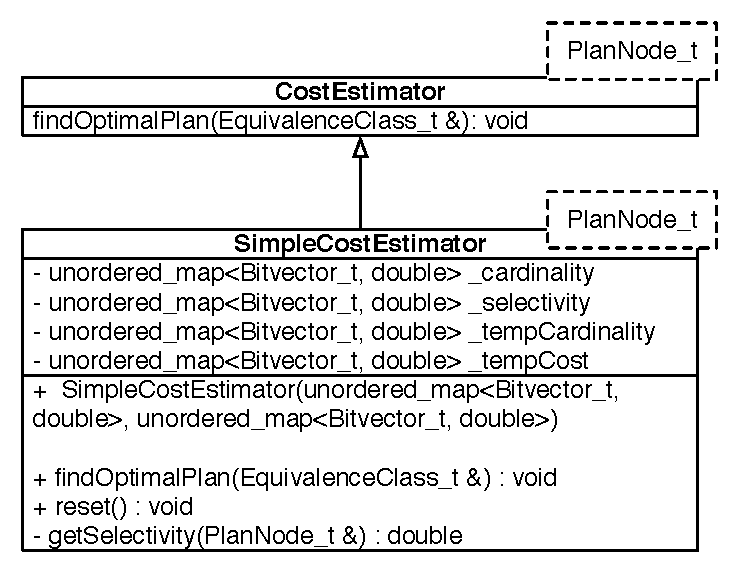
\includegraphics[scale=0.75]{04_Implementierung/00_media/ClassCostEstimation.pdf}
  \caption{Klassendiagramm: Kostenschätzung}
  \label{ClassCostEstimation}
\end{figure}



Die konkrete Implementierung der Kostenfunktion wird in der Klasse \texttt{Simple\-Cost\-Estimator} vorgenommen. In ihrem Konstrukor wird die Kardinalität und die Selektvität von Basis-Relationen und Join-Kanten übergeben. Sie stammen aus der Konfiguration und sind die Grundlage der Berechnung. Die Klasse erfüllt das Interface \texttt{Cost\-Estimator}, das die Methode \texttt{find\-Optimal\-Plan(Equivalence\-Class\_t \&)} vorgibt. Dies ist in Abb. \ref{ClassCostEstimation} zu sehen.

Die Hilfsmethode  \texttt{get\-Selectivity(Plan\-Node\_t \&)} ermittelt die Selektivität für einen Planknoten.


Die Kostenberechnung wird rekursiv durchgeführt. Wie in \ref{PseudocodeCostEstimator} zu sehen, wird für jeden Planknoten, der in der Äquivalenzklasse vorhanden ist, zuerst geprüft, ob es sich um einen \texttt{SCAN} handelt. Wie zuvor beschrieben existieren zwei Operatoren \texttt{JOIN} und \texttt{SCAN}. Es ist nicht möglich, dass einem \texttt{SCAN} ein \texttt{JOIN} untergeordnet ist. 

Somit sind die Kosten für einen \texttt{SCAN} nach unserem Kostenmodell gleich der Kardinalität des \texttt{SCAN}-Planknoten. Falls es sich um keinen \texttt{SCAN} handelt, wird geprüft, ob die linke und die rechte Äuqivalenzklasse einen optimalen Planknoten gefunden haben. Wenn das nicht der Fall ist, wird die Suche nach diesen angestoßen und somit der Rekursion gestartet. Nachdem die optimalen Planknoten für die untergeordneten Äquivalenzklassen gefunden sind, kann die Kardinalität sowie die Kosten für den aktuellen Knoten berechnet werden. Falls die Kosten niedriger sind als die bisher bekannten Kosten für den bisher optimalen Plan, wird der beste Plan neu gesetzt und die optimalen Kosten und die Kardinaltität des Äquivalenzknotens angepasst.



\begin{algorithm}[ht]
\SetAlgoLined
\SetKwFunction{findOptimalPlan}{findOptimalPlan}
\SetKwProg{myalg}{Algorithm}{}{}

\myalg{\findOptimalPlan{EquivalenceClass eq}}{
    \For{PlanNode p in eq.PlanNodes}{
        \If{p.operator == SCAN}{
            eq.best = p
            
            eq.costs = p.cardinality
            
            eq.cardinality = p.cardinality
            
            return
        }
        
        \If{p.left.best == NULL}{
            findOptimalPlan(p.left)
        }
        \If{p.right.best == NULL}{
             findOptimalPlan(p.right)
        }
        
        p.cardinality = p.left.cardinality * p.right.cardinality * p.selectivity
        
        p.cost = p.left.cost + p.right.cost + p.cardinality
        
        \If{p.cost < eq.cost OR eq.cost == NULL}{
            eq.cost = p.cost
            
            eq.cardinality = p.cardinality
            
            eq.best = p
        }
    }
}
\label{PseudocodeCostEstimator}
\caption{Kostenfunktion: SimpleCostEstimator}
\end{algorithm}


\subsection{Erweiterbarkeit der Kostenfunktion}
Diese Implementierung ist nur eine starke Vereinfachung. Sie bezieht nur sehr einfache Parameter in die Berechnung ein. Keine komplexen Kostenfunktionen wurden implementiert. Dank der Modularität des Prototypen ist es möglich, neue, akkuratere Kostenfunktionen zu erstellen und diese auch zu implementieren. Dafür muss ausschließlich das Interface \texttt{Cost\-Estimator} erfüllt werden, das bereits in Abb. \ref{ClassCostEstimation} vorgestellt wurde.


\section{Enumeratoren und Konfiguration von Test}

Die Konfiguration eines Test wird von der Klasse \texttt{Executor} vorgenommen. Iteriert über die Liste der Konfigurationsobjekte, die mit dem \texttt{Configurator} erzeugt wurden. Für jede Regelmenge, die in einem Test festgelegt ist, wird ein eigener initaler Plan erzeugt. Der Enumerator wird mit einer Regelmenge initalisiert. Jetzt kann die Zeitmessung gestartet werden und der initale Plan an den Enumerator übergeben werden. Der Enumerator führt die Regeln aus. Das Ergebnis ist eine expandierte Äquivalenzklasse. Die an die Kostenschätzung weitergegeben wird. Ist hier der optimale Plan ermittelt, stoppt die Zeit und die Messung kann gespeichert werden.



\begin{figure}[ht]
  \centering
  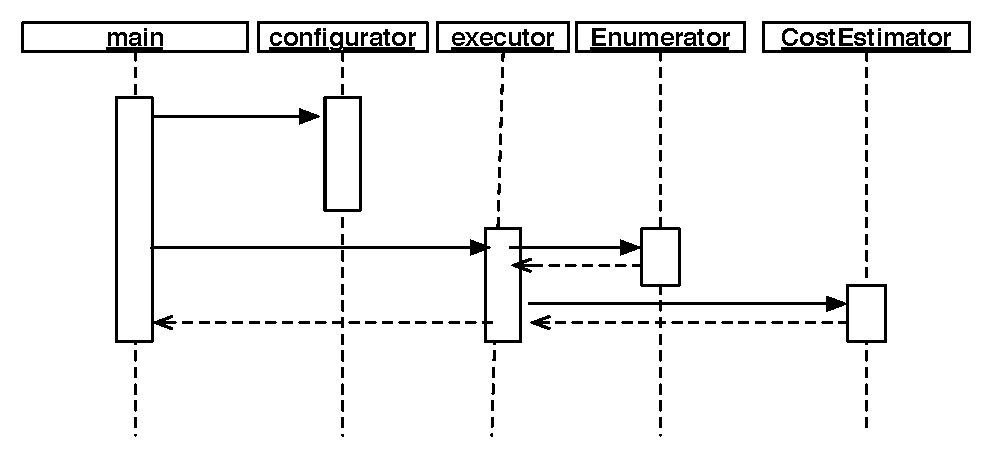
\includegraphics[width=\textwidth]{04_Implementierung/00_media/SequenceDiagramConfiguration.pdf}
  \caption{Sequenzdiagramm: Aufruf von Main zu Enumerator}
  \label{SequenceDiagramConfiguration}
\end{figure}






\section{Organisation und Aufbau}


Das Projekt ist entlang der unterschiedlichen Aufgaben modular organisiert. Unter dem Dach der Anwendung finden sich vier unterschiedliche Sparten, die gemeinsam für das Ausführen des Programms verantwortlich sind: Planknoten und Äuqivalenzklassen, Regeln und Regelsets, Executoren und Services. Die genaue Zuordnung zu den jeweiligen Bereichen ist in Abb. \ref{ProjectOrga} nachvollziehbar.


\begin{figure}[h]
  \centering
  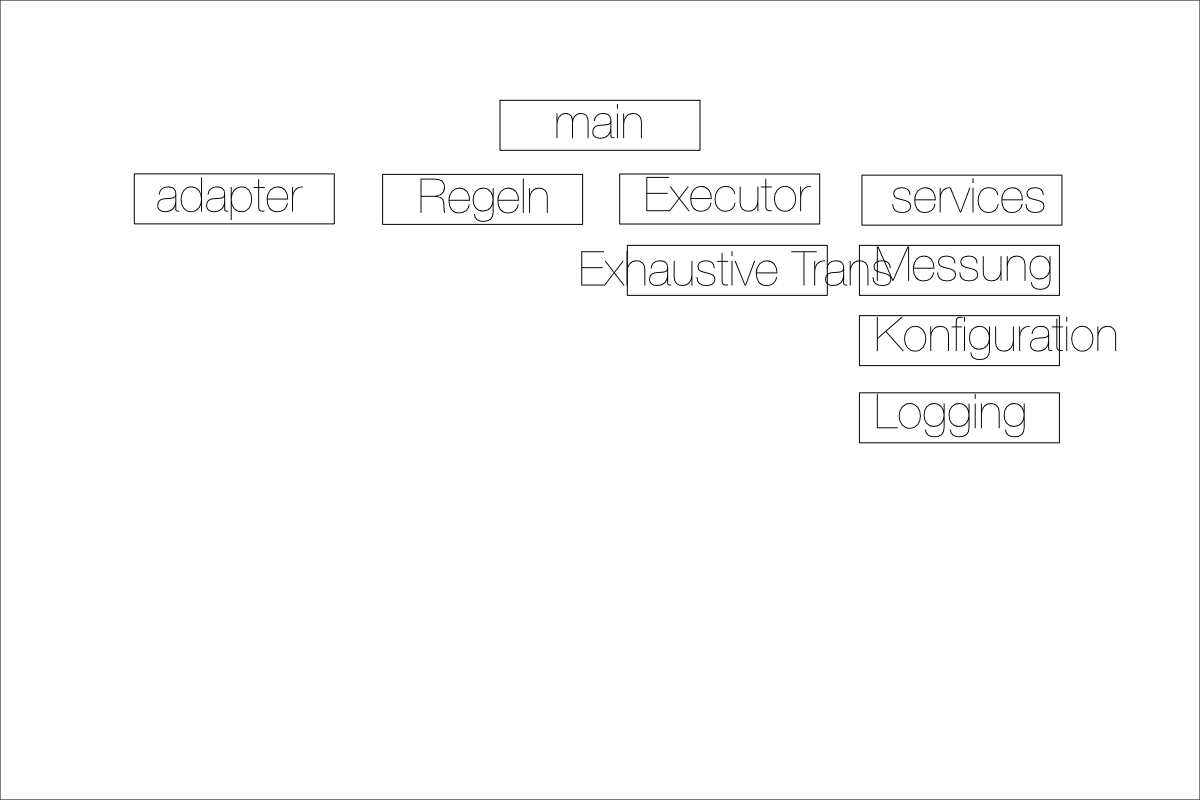
\includegraphics[width=\textwidth]{04_Implementierung/Matrix.png}
  \caption{Projektorganisation}
  \label{ProjectOrga}
\end{figure}

Bei der Ausführung eines Tests  müssen alle Bereiche zusammenarbeiten. Der Service-Bereich und insbesondere das Konfigurationsmodul sind für die konkrete Zusammenstellung der für den Test notwendigen Komponenten verantwortlich. Er entscheidet, welche Regeln zum Einsatz kommen, welcher Exector gewählt wird, welche konkreten Pläne getestet und mit Hilfe welcher Adapter die Daten ein-  bzw. ausgegeben werden. Um zu verstehen, welche Möglichkeiten das implementierte System bietet, sind die einzelnen Komponenten im Folgenden im Detail beschrieben.


\section{Services}

Da für die Ausführung des Programms unterschiedliche Dienstleistungen benötigt werden, die auch in anderen Kontexten relevant sein können, falls das Projekt diese Funktionen im Bereich Services zusammen. Teil des Bereichs ist der Konfigurator, der die Konfiguration der Tests übernimmt, die Zeitmessung und Das Logging von Informationen.

Nicht alle Komponenten wurden selbst entwickelt, beispielsweise wurde beim Logging auf die existierende Library easylogging++ gesetzt.

\subsection{Konfiguration}


\begin{figure}[ht]
  \centering
  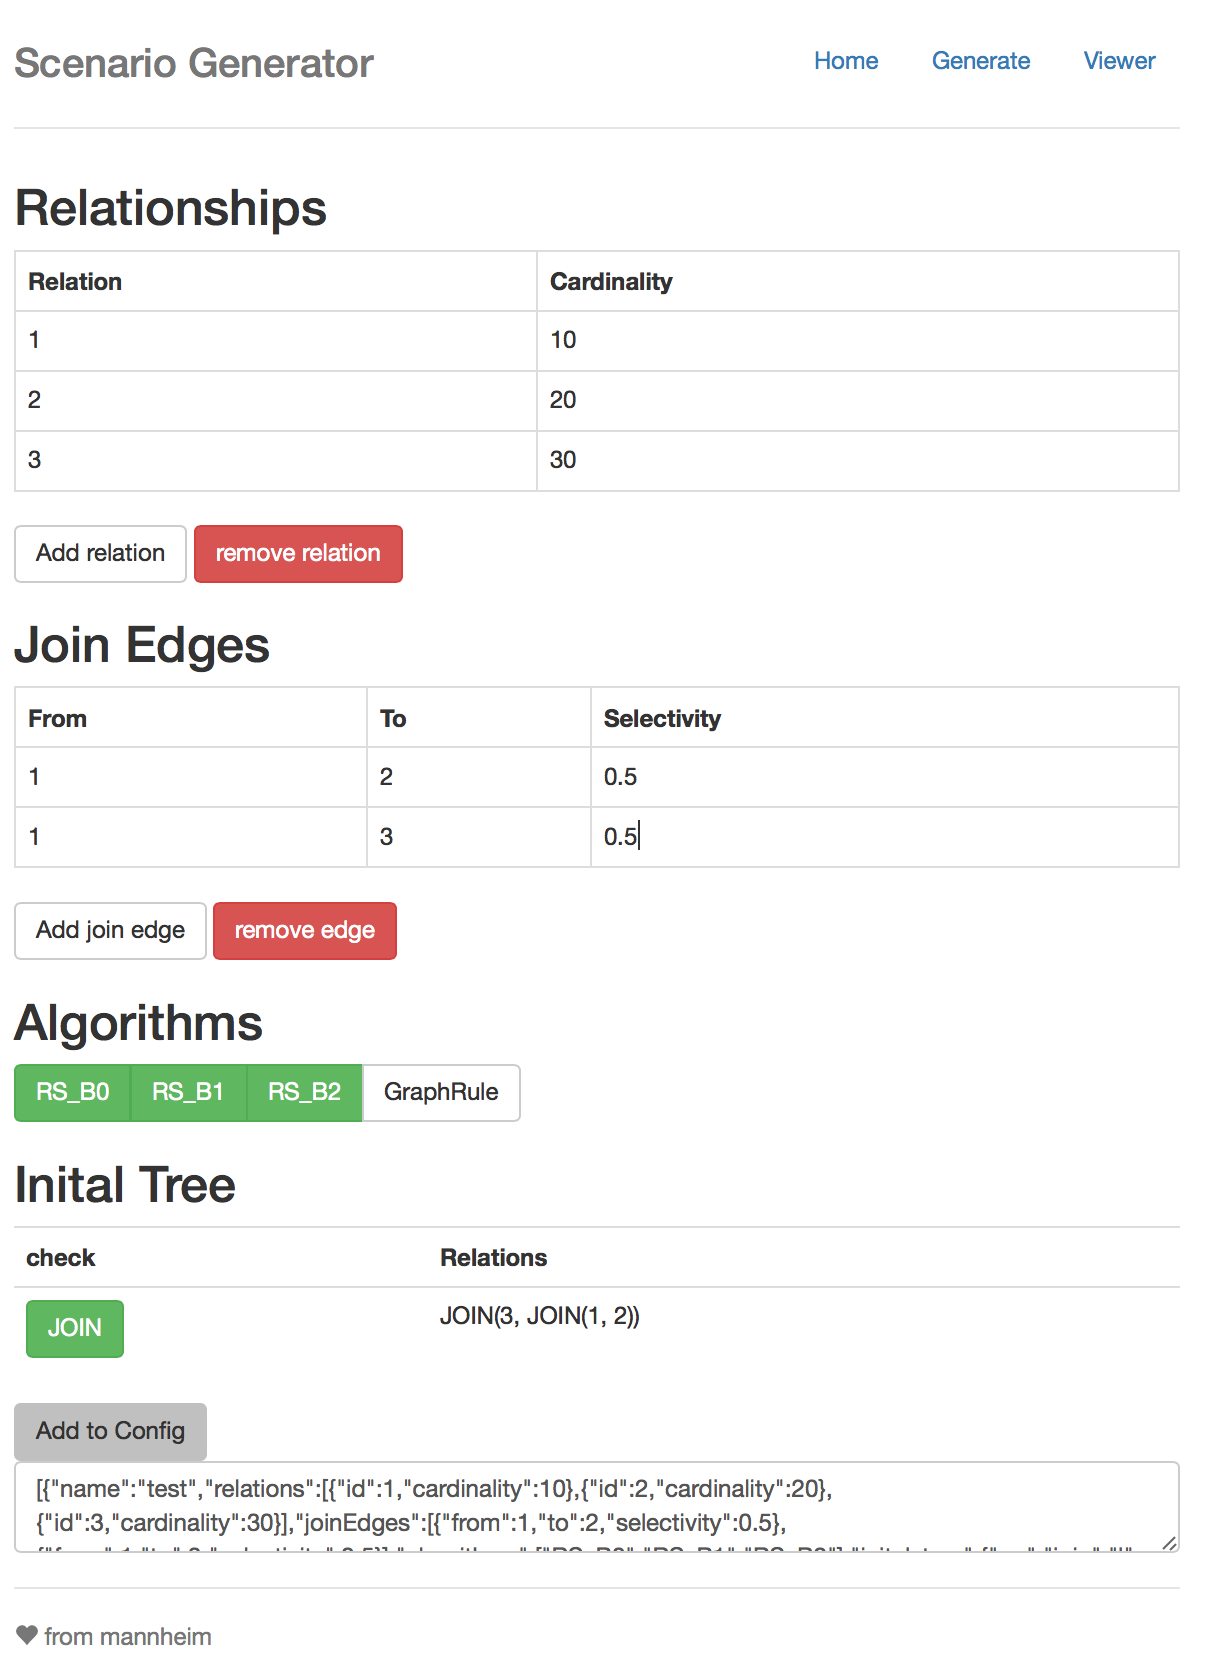
\includegraphics[width=0.5\textwidth]{04_Implementierung/ScenarioGenerator.png}
  \caption{Konfigurationstool: Scenario-Generator}
  \label{ScenarioGenerator}
\end{figure}

Das Konfigurationsmodul besteht aus zwei Komponenten. Auf der einen Seite eine Javascript-HTML Anwendung zur Generierung von Test-Szenarien (vgl. Abb. \ref{ScenarioGenerator}). Mit Hilfe dieser Anwendung können Konfigurationsfiles für den späteren Test erstellt werden. Dieses Konfigurationssystem, das in  zu sehen ist, bietet dem Nutzer die Möglichkeit Relationen mit Kardinalitäten zu erzeugen, Selektivitäten festzulegen und schlussendlich einen initalen Query Tree zu erzeugen. Ebenfalls ist es möglich die verschiedenen Regelsets, die geprüft werden sollen, festzulegen.
Das Ergebnis dieses Moduls ist eine Konfigurationsdatei im JSON Format. Das Tool unterstützt die Erzeugung mehrerer Secenarios in einem Konfigurationsfile. So können mehrere Scenarios in einem Test-Run durchgespielt werden.

Die eigentliche Konfiguration findet in C++ statt. Mit der Library json11 \cite{json11} wird das Konfigurationsfile gelesen. Für jedes Szenario und jedes Regelset wird ein initaler Baum aus Äquivalenzklassen und Planknoten mit einem JSON-Adapter gebildet. Der Exekutor wird gewählt und mit einem Regelset initialisiert. Der initiale Baum wird dem Exekutor übergeben. Nachdem die Regeln angewendet wurden, startet der Konfigurator die Kostenschätzung. Nachdem alle Szenarios abgearbeitet sind, ist das Programm beendet.

\subsection{Zeitmessung}
Wie bereits in Abb. \ref{Ablauf} dargestellt wird die Zeitmessung nach der Konfiguration gestartet. Sobald alle Pläne expandiert sind und die Kosten berechnet sind wird die Messung beendet. Um eine möglichst genaue Messung durchführen zu können, wurde die Uhr \texttt{std::chrono::steady\_clock} verwendet. Diese Uhr ist Teil von C++11. Wie in der Dokumentation \cite{cppreference_2015_clock} beschrieben handelt es sich bei der Uhr um eine monotone Uhr. Die Uhr kann nicht rückwärts laufen, solange die physische Zeit fortfährt. Die Uhr selbst mit der Wall\-Clock\-Time verbunden und ist das passende Werkzeug zur Messung von Intervallen. 

Die Dauer zwischen Start der Expansion und dem Ende der Kostenberechnung wird in Nanosekunden gemessen, um ein möglichst akkurates Ergebnis zu erhalten. Die gemessenen Ergebnisse werden sowohl als Debug-Log in der Konsole ausgegeben, aber auch in einem Log File gespeichert.



\subsection{Logging und Debugging}

Auch zum Debugging wurde eine externe Bibliothek eingesetzt: EasyLogging++ \cite{easylogging}, ein einfach zu bedienendes jedoch hochgradig konfigurierbares Logging Instrument. Gerade die Leichtgewichtigkeit - das Tool besteht nur aus einer Headerklasse -, die einfache Bedienung und Geschwindigkeit gabem den Ausschlag zur Nutzung der Library. Mit Hilfe dieser Library werden debugging Informationen geschrieben, aber auch Zeitmessungen gespeichert, pläne ausgegeben und sonstige Debugging Nachrichten ausgegeben. Insbesondere ist die Unterscheidung zwischen unterschiedlichen Debug\-Leveln wichtig. Auf mehreren Ebenen (INFO, WARNING, DEBUG, etc.) können Informationen ausgegeen werden. Je nachdem welches Level angesprochen ist, werden nur Informationen über dieses ausgegeben. 


\section{Adapter}

Die Implementierung bietet mehrere Adapter, die zur Umwandlung von externen Formaten in eine interne Repräsentationsform oder von einer internen Repräsentationsform in ein externes Format genutzt werden können. Sie bieten die Möglichkeit andere Systeme an das bestehende System anzudocken und sorgen so für den notwendigen Anschluss und die Erweiterbarkeit durch Dritte.

Insgesamt werden drei Adapter mitgeliefert. (1) JSON\-Adapter, (2) String\-Adapter, (3) DOT\-Adapter.

Der Json-Adaper erlaubt des Daten im JSON Format zu importieren und wird beim einlesen des initalen Plans genutzt. Er wandelt auf Basis des Konfigurationsfiles JSON in Planknoten und Äquivalenzklassen um, die dann weiterverarbeitet werden können. Ebenfalls ist es möglich Pläne in JSON auszugeben. Zu diesem Zweck implementiert der Parser auch eine \texttt{dump} Methode.

Neben dem JSON\-Adapter wird auch ein String Adapter verwendet. Er ist für die Ausgabe von Plänen als String verantwortlich. Im Gegensatz zu einem JSON\-Adapter ist die Eingabe von Plänen mit Hilfe dieses Moduls nicht möglich. Auch der DOT\-Adapter erlaubt nur die Ausgabe von Plänen im DOT\-Format. Das zur Generierung von graphischen Ausgaben verwendet werden kann.

Eine weitere Aufgabe eines solchen Adapters kann auch die Übersetzungen von Relationsnamen in Bitvektoren sein. Da das vorliegende System, wie in \ref{sec:Bitvector} beschrieben, Relationen als Bitvektoren abbildet, mag es nützlich sein, Relationsnamen in Bitvektoren zu übersetzen. Für diese Übersetzung sind auch Adapter vorgesehen, die zusätzlich implementiert werden können.




\section{Regeln und Regelsets}

\subsection{Regeln}

\subsection{Regelsets}


\section{Relationen, Planknoten und Äquivalenzklassen}

\subsection{Verwaltung von Relationen}
\label{sec:Bitvector}


\begin{figure}[ht]
  \centering
  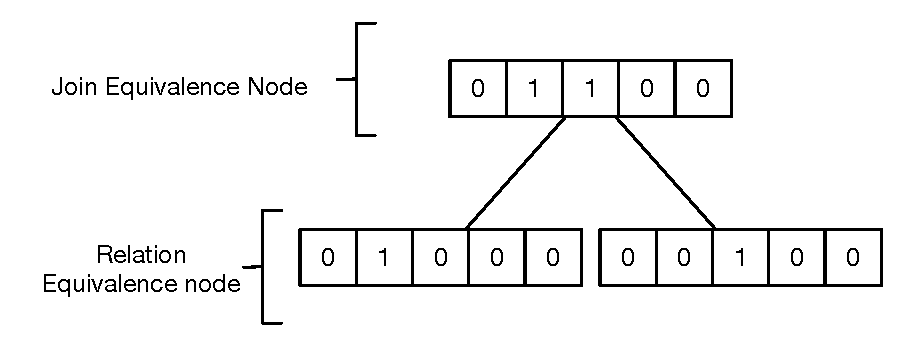
\includegraphics{04_Implementierung/Bitvector.pdf}
  \caption{Bitvekotren als Repräsentation von Relationen oder Joins}
  \label{Bitvektor}
\end{figure}

Die einzelnen Relationen werden mit Hilfe von Bitvektoren repräsentiert. Ein Bitvektor sind mehrere Bits, die entweder $TRUE$ also $1$ oder $FALSE$ also $0$ sein können. Ist das n-te Bit eines Bitvektors gesetzt, so repräsentiert dieses Bit die n-te Relation. Beispielsweise bezeichnet der Bitvektor $010000000$ die Relation mit dem Namen $1$. Mit Hilfe des Bitvektors können auch mehrere Relationen gespeichert werden $01010000000$ bezeichnet folglich die Relation mit dem Name $1$ und die Relation mit dem Namen $3$. Für die durchgeführten Berechnungen ist es nicht notwendig, dass eine Relation mit ihrem tatsächlichen Namen bekannt ist. Es reicht eine Bezeichnung mit Hilfe von Nummern aus.

Vorteil für die Verwendung von Bitvektoren ist, dass einfach Mengenoperationen durchgeführt werden können. So kann einfach geprüft werden, ob Äquivalenzklassen gemeinsame JOIN Kanten besitzen oder neue Relationen einer Äquivalenzklasse hinzugefügt werden. (vgl. Abb. \ref{Bitvector}) Dies ist besonders effizient, da nur Bits und keine komplexen Objekte wie Strings verarbeitet werden müssen.


Für externe Systeme kann es daher notwendig sein, dass Relationsnamen mit Hilfe eines Adapters übersetzt werden. Die genau Funktionsweise eines solchen Adapters wird in diesem Kapitel genauer beschrieben.




\subsection{Planknoten und Äquivalenzklassen}





\begin{figure}[h]
  \centering
  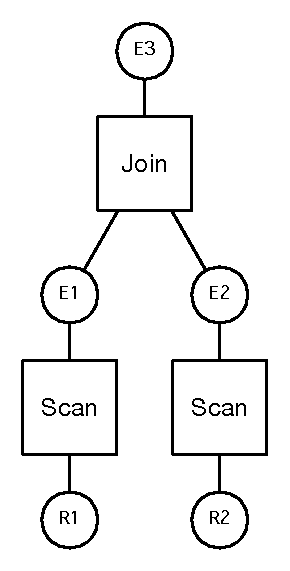
\includegraphics{04_Implementierung/JoinScan.pdf}
  \caption{Planknoten und Äquivalenzklassen}
  \label{PlanAequi}
\end{figure}

Zu  Beginn steht die Struktur in der Pläne gespeichert werden. Diese Struktur wird durch andere Komponenten bearbeitet und ausgewertet und stellt somit das Werkstück bei der Verarbeitung dar.

Ähnlich wie in anderen System kommen in der aktuellen Implementierung Äquivalenzklassen und Planknoten zum Einsatz. Äquivalenzklassen repräsentieren ein Set von unterschiedlichen, jedoch äquivalenten Planknoten. Mit Hilfe von Äquivalenzklassen und Planknoten kann die Information über alle möglichen Äquivalenten Pläne gespeichert werden. Sie können also den gesamten Search Space abbilden.
 Aufgabe eines Planknotens ist es einen Operator zu repräsentieren. Jeder Operator kann mehrere Parameter besitzen. Im konkreten Fall sind zwei Operatoren implementiert: JOINs und SCANs. Scans zeichnen sich dadurch aus, dass sie immer genau eine Relation lesen. Folglich haben Sie nur einen Parameter, um die Relation zu übergeben. Bei Joins gibt es immer genau zwei Parameter. Beide Parameter repräsentieren Datenströme, die mit Hilfe des Joins in einen gemeinsamen Datenstrom kombiniert werden.

Die kleinste im System mögliche Datenstruktur ist ein Scan. Er besteht aus einer Äquivalenzklasse, die die Relation repräsentiert. Auf sie wird ein Planknoten angewendet mit dem Operator SCAN. Dieser Planknoten ist selbst wieder Teil einer Äuqivalenzklasse. Eine solche Datenstruktur ist im linken Teil der Abbildung \ref{PlanAequi} zu finden.

Kombiniert man zwei dieser SCANs mit einem JOIN so erhält man die kleinste mögliche Struktur, die einen JOIN beinhaltet. Dies ist in Abb. \ref{PlanAequi} zu sehen. In diesem konkreten Fall ist noch keine Transformation auf den bestehenden Graphen angewendet worden. Es existieren also noch keine alternativen Planknoten. Eine solche Transformation könnte beispielsweise zur Folge habe, dass neben dem bisher bestehenden JOIN Knoten ein neuer JOIN Knoten erzeugt wird, der die beiden untergeordneten Relationen in umgekehrter Reihenfolge joint.


\subsection{Konkrete Implementierung}

Die konkrete Implementierung der Äquivalenzklasse sieht vor, wie in Abb. \ref{EquivalenceClassDiagram} zu erkennen, dass für jede Äquivalenzklasse die darin aggregierten Relationen sowie deren Nachbarn gespeichert werden. Ebenfalls wird der erste, letzte und kosteneffektivste Planknoten gespeichert. Außerdem kann festgehalten werden, ob eine Äquivalenzklasse bereits $explored$, also erforscht, ist. 






\subsection{Exektuoren}










\section{Regeln und Regelsets}


Eine entscheidende Komponente sind Regeln und Regelsets. Mehrere Regeln werden in einem Regelset zusammengefasst. Ein Regelset ist eine Instanz der abstrakten Klasse $RuleSet$, die die Methode $getRules()$ vorgibt, mit deren Hilfe ein Vektor von Regeln ausgegeben wird. Je nach Regelset können andere Regeln vorhanden sein.







\subsubsection{Organisation von Regeln}


\begin{figure}[h]
  \centering
  \includegraphics[width=\textwidth]{04_Implementierung/Rules.pdf}
  \caption{Regeln und Regelsets Klassendiagramm}
  \label{RuleClassDiagram}
\end{figure}


Auch bei den Regeln erben alle Regeln direkt oder - und das ist neu - indirekt von der Klasse $Rule$. Die Organisation der Klassen ist in Abb. \ref{RuleClassDiagram} dargestellt. Insgesamt wird zwischen den Regeln auf drei Ebenen unterschieden: 

$Commutativity$, $LeftAssociativity$ und $RighAssociativity$ bilden die erste Ebene der Regeln. Sie kommen in Verbindung mit den RuleSets $RS_0$ und $RS_1$ zum Einsatz.

Auf dem zweiten Level, diese Klassen sind mit dem Zusatz $B2$ gekennzeichnet, finden sich $Commutativity_B2$, $LeftAssociativity_B2$, $RighAssociativity_B2$ und $Exchange_B2$. Diese Regeln sind für das Regelset $RS_2$ notwendig und erlauben es andere Regeln zu deaktivieren. Da die Deaktivierung von Regeln eine Erweiterung darstellt, erben Kommutativität und Assoziativität von ihren Verwandten aus $RS_0$ bzw. $RS_1$. Da die Exchange Regel neu hinzukommt, erbt diese direkt von Rule.

Auf dem dritten Level findet sich die $GraphRule$. Sie ersetzt andere Regeln und ist im RuleSet $GraphRuleSet$ abgebildet.


Ähnlich wie bei Starburst bestehen Regel aus zwei Teilen. Auf der einen Seite wird geprüft, ob eine Regel zur Anwendung kommen kann. Dies geschieht mit der Methode $isApplicable$ auf der anderen Seite gibt es die Methode $apply$, die immer einen äquivalenten Planknoten zurückliefert. Mit Hilfe dieses Prinzips wurden alle Regeln implementiert. Das einheitliche Interface erlaubt es, dass Regeln in Regelsets gebündelt werden können.


\subsubsection{Erweiterbarkeit von Regeln}

Die Erweiterbarkeit ist auf mehreren Ebenen sichergestellt. Auf der einen Seite können neue Regeln erzeugt werden. Sobald diese die Form der abstrakten Klasse $Rule$ übernehmen, können sie in Regelsets zum Einsatz kommen. Ein Beispiel für eine solche Erweiterung ist die Regel $GraphRule$. Sie wurde später der entwickelten Lösung hinzugefügt. Das neue RuleSet $GraphRuleSet$ beinhaltet in diesem speziellen Fall nur eine Regel.

Eine weitere Möglichkeit zur Erweiterung wurde ebenfalls von $GraphRule$ genutzt. GraphRule gibt nicht nur einen einzelnen neuen Planknoten zurück, sondern übergibt gleich einen vollständig expandierten Baum. Auch diese Anforderung konnte ohne Veränderung des Interfaces umgesetzt werden. Da der Planknoten ein $next$ Attribut besitzt, das den vorhergehenden mit dem nächsten Knoten verbindet, können Ketten von neuen Knoten gebildet werden. Diese Ketten werden im Falle der $GraphRule$ zurückgegeben ohne dabei das Interface zu brechen.

Neben den vorgegebenen  Methoden können auch weitere Methoden für eine Regel implementiert werden. Dies ist beispielsweise bei $GraphRule$ notwendig gewesen. Hier ist es erforderlich, dass der Graph zuerst partitioniert wird, dann ConnectedComponents gefunden und schlussendlich ein Baum zurückgegeben wird. Auch dies ist innerhalb der Rules möglich.

Eine weitere Möglichkeit zur Erweiterung ist durch Templates gegeben. Template ist eine Funktion von C++ mit deren Hilfe Funktionen und Klassen mit generischen Typen arbeiten können. Dadurch ist es einer Funktion der einen Klasse möglich viele unterschiedliche Typen zu unterstützen ohne die Funktion oder die Klasse bearbeiten zu müssen. Im konkreten Fall der Regeln werden zwei dieser generischen Typen verwendet: $PlanNode$ und $Operations$. Es wird somit möglich die Klassen des Planknotens und die möglichen Operationen, die für diese Planknoten möglich sind zu ersetzen, ohne Funktionen und Klassen verändern zu können.

\subsubsection{Erweiterbarkeit von Regelsets}

Auch die Erweiterung von Regelsets ist möglich. Mit Hilfe neuer Regelsets, kann eine neue Reihenfolge bei der Ausführung definiert werden. Eine weitere Priorisierung von Regeln ist bisher nicht vorgesehen. Es ist jedoch möglich mit Hilfe der Methode $getRules()$, die für jedes Regelset implementiert ist, eine spezielle Priorisierung zu implementieren. 

Neben der Priorisierung sind auch neue Zusammenstellungen möglich. Beispielsweise ist der Unterschied zwischen $RS_0$ und $RS_1$ nur, dass eine Assoziativ-Regel weggelassen wurde. Ein Mix von alten und neuen Regeln ist möglich.

Wird ein neues Regelset erstellt, ist es nicht nur notwendig eine neue Regelset Klasse zu erstellen, sondern auch diese für das Ausführen im Executor anzumelden. Der Executor muss also ebenfalls angepasst werden.



\subsection{Ausführung von Regeln}

Das eigentliche Ausführen der Regeln wird durch einen XY durchgeführt. Im konkreten Fall kommt hier der Algorithmus ExhaustiveTransformation zum Einsatz. Der Algorithmus startet mit einer Äquivalenzklasse. Innerhalb dieser Äquivalenzklasse werden die Regeln, die durch ein Regelset vorgegeben sind auf einem PlanKnoten ausgeführt. Die Ausführung geschieht hierbei zuerst auf den Oberen Ebenen und setzt sich dann auf den Kindern eines Knoten fort. Somit können bei der Transformation eines gegebenen Baums alle Regeln auf andere Bäume angewendet werden.

Wichtig ist hierbei zu bemerken, dass dieser Algorithmus immer zuerst prüft, ob eine Regel auch tatsächlich für die Anwendung geeignet ist und dann erst der Algorithmus ausgeführt wird. Neben der eigentlichen Eignung wird auch geprüft, ob eine Äquivalenzklasse bereits vollständig expandiert wurde. Falls dies der Fall ist, wird von einer weiteren Anwendung von Regeln abgesehen. Diese Funktion kann insbesondere Vorteile bei der Implementierung von neuen Regelsets bieten. Nutzt ein gegebenes Regelset die Möglichkeit nicht nur einen neuen Planknoten zu generieren, sondern gleich mehrere Planknoten zu erstellen und auch in diesem Zusammenhang bereits mehrere Kinder-Knoten zu erstellen, kann die Reihenfolge der Expansion von Äuqivalenzklassen geändert werden. Die einzelnen Äquivalenzklassen, die bereits durch eine Regel expandiert wurden, werden als solche markiert und die bisher vorhandenen Regeln werden nicht mehr ausgeführt.


\section{Kostenschätzung und statistische Informationen}



Die Kostenschätzung zur Suche des optimalen Plans geschieht bei der vorliegenden Implementierung in einem eigenen Kostenschätzungsmodul.Teil des Kostenmoduls ist ein Katalog innerhalb dessen Informationen über Selektivität von JOINs und Kardinalitäten von Relationen gespeichert sind. Diese Informationen werden aus dem Katalog mit Hilfe des Kostenschätzers ausgelesen und die Kosten für einen Planknoten berechnet.

Die Berechnung der Kardinalität findet bottom up statt. Für jede Äquivalenzklasse wird die optimale Kardinalität berechnet und gespeichert. Der Planknoten mit dessen Hilfe diese optimale Kardinalität erreicht wird, wird als bester Planknoten markiert. Folgt man dem Pfad der besten Planknoten ergibt sich der kostenoptimale Baum an Planknoten. Die Berechnung sieht vor, dass immer die Selektivität eines Operators mit dem Produkt der Kardinalität der Eingabeparameter multipliziert wird. Beispielsweise wird auf der untersten Ebene - der Ebene der Scans - für eine gegebene Relation die Kardinalität mit der Selektivität von 1 multipliziert, da die gesamte Relation verarbeitet werden muss. Bei einem Join können komplexere Situationen auftreten. Zuerst wird das Produkt der Kardinalität der Eingabe Parameter berechnet. Diese kann dann mit der 
Selektivität multipliziert werden. Das Produkt der Kardinalitäten repräsentiert in diesem Falle die Kardinalität des möglichen Kreuzproduktes, das mit Hilfe von Selektoren eingeschränkt wird.



\subsection{Zusammenfassung}

Gerade im Bereich der Regeln ist klar zu erkennen, dass die SOLID Prinzipien eingehalten wurden. Hier ist jede Klasse nur für genau eine Aufgabe zuständig. Ein hohes Maß an Kohäsion konnte erreicht werden. Die Regelklassen  sind offen für Erweiterungen, jedoch geschlossen für Modifikationen. Dies wird insbesondere bei der Erweiterung mit Hilfe des Regelsets $GraphRuleSet$ deutlich. Auch das Liskov Substitutionsprinzip wurde eingehalten. Alle Klassen verhalten sich nach außen gleich und liefern dasselbe Ergebnis, einen Planknoten, zurück. 


\subsection{Unterschiede zu Volcano und Pyro(J)}

Einer der fundamentalen Unterschiede zwischen Pyro bzw. Volcano zur hier vorgestellten Implementierung ist, dass sowohl Volcano als auch Pyro vollständige Optimierer sind. Sie erstellen basierend auf einer Anfrage einen physischen Plan, der dann weiterverarbeitet werden kann. Im Gegensatz dazu wird für diese Masterarbeit nur das Anpassen der Join-Reihenfolge betrachtet und daher auch nur das Anpassen der Join-Reihenfolge implementiert.


Ebenfalls wird von Volcano und Pyro immer ein physischer Plan erzeugt. Dies geschieht in dieser Implementierung nicht. Es werden somit nur für die logischen Pläne Alternativen gefunden und aus diesen Alternativen der günstigste Plan ausgewählt. Dies geschieht, da für die Überprüfung der Regelsets RS-B0, RS-B1, RS-B2 und GraphRule keine pysischen Pläne notwendig sind. Die unterschiedlichen Regelmengen widmen sich nicht dem Berechnen von physischen Alternativen, sondern dem Finden alternativer Join-Reihenfolgen. Falls alle Pläne gefunden werden, wäre der Aufwand für die Umwandlung in physische Pläne für alle Regelmengen gleich. Daher trägt die Umwandlung und weitere Expansion nicht zu Unterschieden in der Expansionsgeschwindigkeit bei.

Ein weiterer Unterschied zu Volcano ist, dass alle Pläne direkt berechnet werden und  anschließend aus allen Plänen der günstigste Plan ausgewählt wird. Volcano berechnet zuerst einen Plan und wählt dann aus der Menge der physischen Pläne den günstigsten aus, bevor der nächste logische Plan berechnet wird. Nur falls ein günstigerer Plan gefunden wird, wird dieser auch im Speicher behalten. Im Gegensatz zu diesem sehr ressourcensparenden Verfahren setzt Pyro und die eigen Implementierung auf Pläne die dauerhaft vorgehalten werden. Dies erleichtert das Debugging, da alle Pläne jederzeit betrachtet werden können, erhöht aber den Verbrauch an Arbeitsspeicher.

Neben diesen konzeptionellen Unterschieden setzt die implementierte Lösung wie Pyro oder Volcano auf C++ als Programmiersprache). Im Gegensatz zu diesen Implementierungen setzt PyroJ auf Java und die Java Plattform, die per se mit schlecht beeinflussbaren Faktoren wie Garbage Collection, Virtuellen Maschinen und JIT-Compilern zu kämpfen hat. Wie bereits in Kapitel \ref{} besprochen, mussten bei den Messungen mit PyroJ diverse Parameter gesetzt werden, um überhaupt reproduzierbare Ergebnisse zu erzeugen. Um solchen Problemen vorzubeugen, wurde vollständig auf C++ für die Implementierung gesetzt. Da der Code zur Laufzeit bereits vollständig kompiliert ist, können Probleme durch einen JIT Compiler und Optimierungen zur Laufzeit ausgeschlossen werden. Unterbrechungen durch eine Garbage Collection können nicht auftreten, da keine vorhanden sind.
